% Homework 3   for ENGR 1120 020 120 - Tristan Hill - Fall 2014 - Spring 2020
% 
% Introduction to MATLAB 
%
%  Robot Simulator - Reactive Behaviors

% Document settings
\documentclass[11pt]{article}
\usepackage[margin=1in]{geometry}
\usepackage[pdftex]{graphicx}
\usepackage{multirow}
\usepackage{setspace}
\usepackage{hyperref}
\usepackage{color,soul}
\usepackage{fancyvrb}
\usepackage{framed}
\usepackage{wasysym}
\usepackage{multicol}

\pagestyle{plain}
\setlength\parindent{0pt}
\hypersetup{
    bookmarks=true,         % show bookmarks bar?
    unicode=false,          % non-Latin characters in Acrobat’s bookmarks
    pdftoolbar=true,        % show Acrobat’s toolbar?
    pdfmenubar=true,        % show Acrobat’s menu?
    pdffitwindow=false,     % window fit to page when opened
    pdfstartview={FitH},    % fits the width of the page to the window
    pdftitle={My title},    % title
    pdfauthor={Author},     % author
    pdfsubject={Subject},   % subject of the document
    pdfcreator={Creator},   % creator of the document
    pdfproducer={Producer}, % producer of the document
    pdfkeywords={keyword1} {key2} {key3}, % list of keywords
    pdfnewwindow=true,      % links in new window
    colorlinks=true,       % false: boxed links; true: colored links
    linkcolor=red,          % color of internal links (change box color with linkbordercolor)
    citecolor=green,        % color of links to bibliography
    filecolor=magenta,      % color of file links
    urlcolor=blue           % color of external links
}

\newcommand{\VSpaceSize}{2mm} 
\newcommand{\HSpaceSize}{2mm} 
\newcommand{\secNum}{GSET: Programming}
\newcommand{\assnType}{Project}
\newcommand{\assnTitle}{Robo Sim - A Mobile Robot Simulator}
\newcommand{\assnNum}{1} 
\newcommand{\currTerm}{Summer 2022}
\newcommand{\VER}{2.0 }


\definecolor{mygray}{rgb}{.6, .6, .6}

\setulcolor{red} 
\setstcolor{green} 
\sethlcolor{mygray} 

\begin{document}


	\textbf{\LARGE ENGR \hspace{2mm}\secNum \hspace{1mm} - \hspace{1mm} \currTerm} \\\\
	\textbf{\LARGE \assnType \hspace{1mm}  \assnNum : \assnTitle}\\

         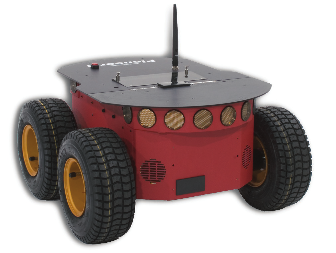
\includegraphics[scale=0.5]{hw2_fig1.png}

	\begin{description}
		
		\item [\textbf{Your Mission}]\textbf{:} \\\\
		You have been given a mobile robot simulator called {\it robo\_sim}. You are going to teach the a robot to navigate through a set of reactive behaviors. You will program the logic used by the robot to interpret sensor data and make decisions. The objective is to train a smart robot that can escape the arena in the least time possible. You will be competing against your peers to make the fastest and safest robot.    

		\item [\textbf{The Robot}]\textbf{:} \\\\
		The robot is very simple and it is modeled as a circular disc with inertia, however it is shown as an arrow to indicate the heading. You can control where the robot drives by choosing throttle and the steering angle. The robot has mass, and therefore momentum, so if you get up to speed you might not be able to slow down in time. The throttle corresponds to a {\it Force} in the forward direction and the steering to a angular {\it Velocity}. 

		\item [\textbf{The Laser Ranger}]\textbf{:} \\\\
		The robot experiences the environment through a sensor called a {\it laser ranger}. This is a special laser that can measure distance. Your robot uses this laser to make 7 measurements separated by 30 degrees in a 180  degree span. The resulting data is essentially coarse polar data. This is used to see obstacles in the path of the robot.			

		\item [\textbf{The Arena}]\textbf{:} \\\\
		The Robot is placed in an environment with obstacles in it and the robot's goal is to escape the arena (shown as a box). However, if you crash into any objects, your robot will be destroyed. In version \VER you are given the option to use a hardcoded map, or create a map using the {\it ginput()} function.
			
		\item [\textbf{The Code}]\textbf{:} \\\\
		The MATLAB code behind the Robot Simulator is complex. However, most of it has been written for you. You will be asked to modify the portion which describes the robots reactive behaviors. Also you will be asked to make a few changes to the simulator code structure. The code can be found on Github \href{https://github.com/thillRobot/robo\_sim}{here}. Click the {\it code} button and download the entire package. Make sure to extract it {\it before} you run or modify it. Stay tuned for updates and revisions of the simulator.

\newpage

		\item [\textbf{The Assignment}]\textbf{:} \\\\
		
		\begin{enumerate}
			\item Teach the robot {\it at least} 5 independent reactive behaviors. These can be as simple or as complex as you would like. The possibilities are endless. Keep in mind you are want to escape quickly but not crash. In version 1.2 the behaviors are currently programmed in the file 'robot\_decide.m'. \\\\
		
			\item Stay Tuned for More...
		\end{enumerate}

			


    \end{description}
          
 
\newpage


\end{document}



